\chapter{Results, Discussion and Conclusion}
\label{resultanddiscussion}
In this chapter, the results of the testing phase will be shown. Further, the design decisions that were made based on these results will be discussed.
 
\section{Arithmetic}
During the system testing phase, extensive testing was done on the performance of different arithmetic algorithms. The performance of each algorithm was measured by toggling one of the GPIO pins to a HIGH state at the beginning of the calculation and resetting it back to LOW as soon as the calculation was done. This way, the processing time could be measured with an Oscilloscope.
It is important to note that the time limit for the real time loop was set to 100$\mu$s. All steps prior to the floating point calculation were measured to use 40$\mu$s of time.
 
\subsection{Floating point arithmetic}
First, the floating point algorithm was tested. This algorithm introduces a cumulating rounding error into the calculation, but had the advantage that the calculation done within the real-time loop is as small as possible. The time measurement with the Oscilloscope showed a calculation time of 40.2$\mu$s. This leaves 59.8$\mu$s time for other steps. When considering the previously measured time of 40$\mu$s for the steps needed prior to the floating point calculation, this leaves a time buffer of 19.8$\mu$s. The measurement result is shown in Figure \ref{ResArithmetic}.
 
\subsection{Fractional arithmetic}
Second, an algorithm was tested using fractional arithmetic. This algorithm had the big advantage that it did not introduce a cumulating rounding error into the calculation of the desired steps. The measurement of this calculation, as shown in Figure \ref{ResArithmetic}, resulted in a calculation time of 55$\mu$s. With the additional 40$\mu$s, while still being within the specification, this algorithm only leaves 5$\mu$s of buffer to the real time criteria.
 
\subsection{Discussion}
Based on the previously done measurements, both algorithms will be calculated within the time limit of 100$\mu$s. However, the fractional arithmetic only leaves 5$\mu$s of buffer, bevor breaking the real time limitation. This would render the solution of the algorithm invalid and one complete calculation cycle would be missed by the system. For this reason, a real time violation has to be avoided.
Based on this, the floating point algorithm was chosen to be implemented into the system. However, further tests have to show if the accumulation of the rounding error of this algorithm has a significant impact on the performance of the Electronic Lead screw.
 
\begin{figure}
    \begin{center}
    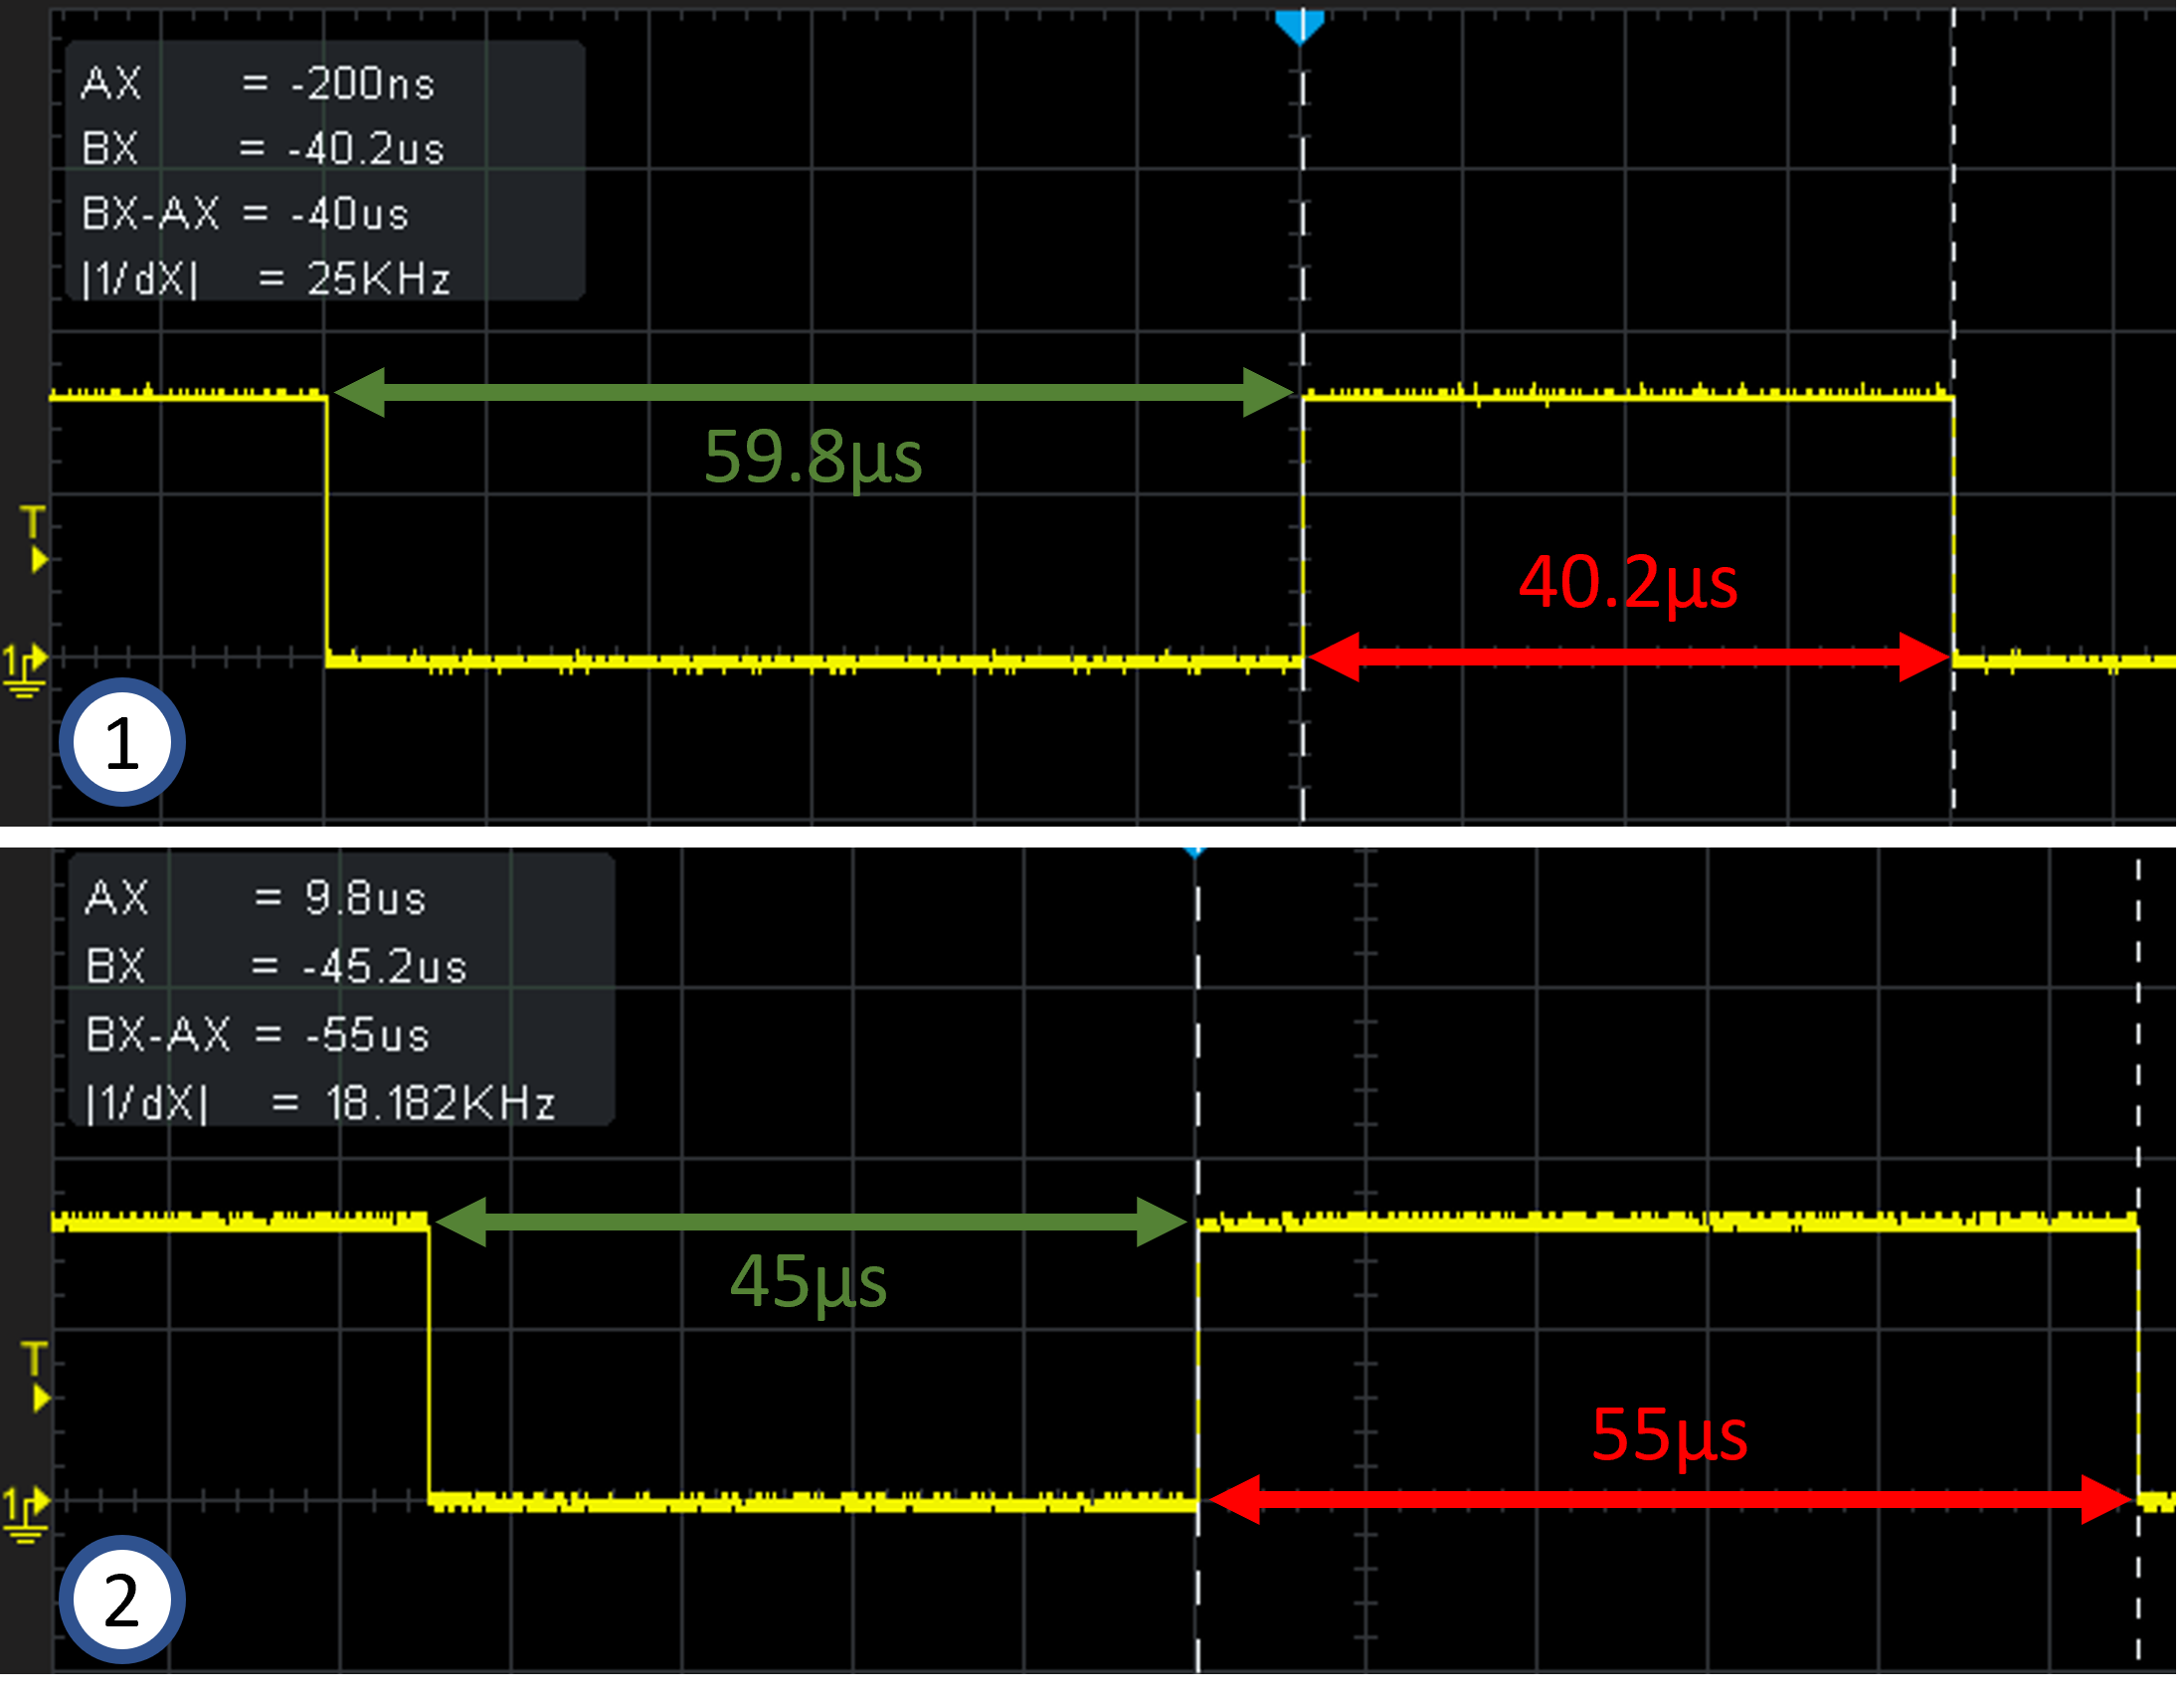
\includegraphics[width=12cm]{Pictures/ResArithmetic.png}
    \caption[Results of the algorithm testing]{Results of the algorithm testing; 1 - Floating point algorithm, 2 - Fractional arithmetic, red - Time needed for the calculation, green - Time needed for the calculation, blue - Time available for other calculation steps}
    \label{ResArithmetic}
    \end{center}
\end{figure}
 
 
\section{Turning}
The test of the normal turning performance of the system was part of the integration test. It was aimed to test both material removal performance and surface quality. As shown in Table \ref{Tab material removal performance} the system performed good up to a feed rate of 0.17 mm/rev. At 0.19 mm/rev the test was canceled because the RPM of the main spindle decreased by $\sim$200rpm.
 
\begin{table}
    \centering
     \begin{tabular}{||c|c|c|c||}
        \hline
        Test. Nr. & Depth of cut & Feed & Success\\ [0.5ex]
        \hline\hline
        1 & 1 mm      & 0.09 mm/rev      & good      \\
        2 & 1 mm      & 0.11 mm/rev      & good      \\
        3 & 1 mm      & 0.13 mm/rev      & good      \\
        4 & 1 mm      & 0.15 mm/rev      & good      \\
        5 & 1 mm      & 0.17 mm/rev      & good      \\
        6 & 1 mm      & 0.19 mm/rev      & canceled  \\[1ex]
        \hline
     \end{tabular}
     \caption{Results material removal performance}
     \label{Tab material removal performance}
\end{table}
 
As shown in table \ref{Tab surface quality testing} the test for surface quality was also performed with a fixed depth of cut and a variable feed rate. With decreasing feed rate, the surface quality was improving consistently, up to a point of 0.05 mm/rev. As soon as the feed was lowered below this point, the surface of the part became blunt. However, it is important to note that the surface quality was determined by eye. This was done because no tool was available to measure the surface quality after each cut.
 
\begin{table}
    \centering
     \begin{tabular}{||c|c|c|c||}
        \hline
        Test. Nr. & Depth of cut & Feed & Success\\ [0.5ex]
        \hline\hline
        1 & 0.05 mm      & 0.09 mm/rev      & ok      \\
        2 & 0.05 mm      & 0.08 mm/rev      & ok      \\
        3 & 0.05 mm      & 0.07 mm/rev      & ok      \\
        4 & 0.05 mm      & 0.06 mm/rev      & ok      \\
        5 & 0.05 mm      & 0.05 mm/rev      & good    \\
        6 & 0.05 mm      & 0.04 mm/rev      & blunt  \\[1ex]
        \hline
     \end{tabular}
     \caption{Results of the surface quality testing}
     \label{Tab surface quality testing}
\end{table}
 
\section{Threading}
The testing of the threading performance of the system was done on two example threads. These threads were chosen, because tools were available to measure the thread precision objectively. Further, it was essential to test both the metric mode of the machine and the transformation into the imperial unit system. In figure \ref{ResThread} the final result of both threading tests and the previous surface quality test is shown. Both, the imperial thread and the metric thread, were within the specifications of corresponding thread gauges. This proofed the capability of the machine to transform its motion calculation into another unit system. Further, it was shown that the impact of the cumulating rounding error introduced by the floating point algorithm on normal threading operations is insignificant.
 
\begin{figure}
    \begin{center}
    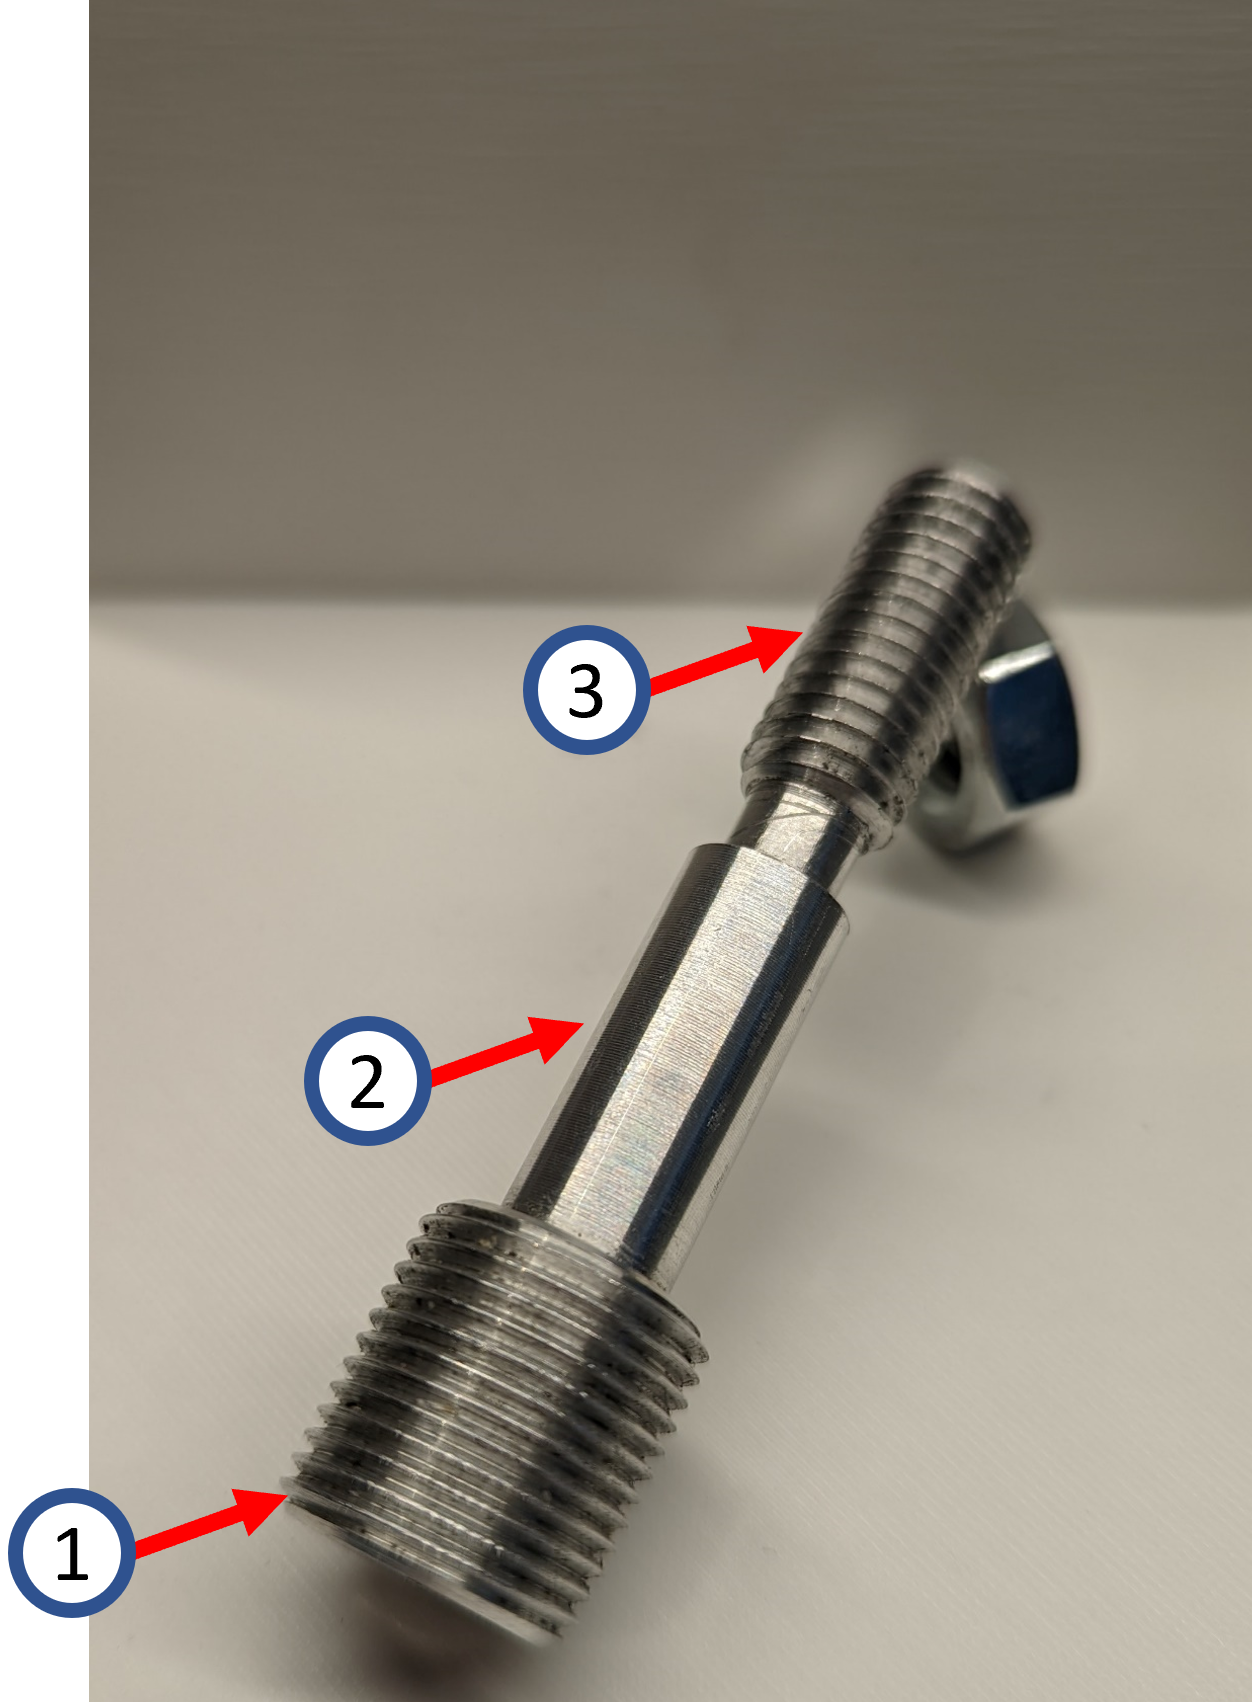
\includegraphics[width=12cm]{Pictures/ResThreadSurf.png}
    \caption[Results of the threading and surface quality test]{Results of the threading and surface quality test; 1 - 3/8" 19G thread, 2 - best surface quality, 3 - M8x1.25 thread}
    \label{ResThread}
    \end{center}
\end{figure}
 
\section{Conclusion}
During the testing, the Electronic Lead screw system has proven to meet the initial defined requirements. Further, this system shows to be a very valuable addition to this lathe. It enables the operator to use a wider range of feeds while reducing the setup time of the machine significant. This increases the capability of a small lathe like the Emco Compact 8 to a point where it is a good addition for every home metal workshop.
 
 

